\chapter{Perturbation Theory}
\label{projection}

This chapter will treat perturbation theory, as the title indicates, and it is mainly based on the work in Ref. \cite{realeff}.\\
\\
The many-body Schr\" odinger equation is rather difficult to solve. 
Even a two body problem is a rather complicated system to solve, that is why
we have to come up with approximated methods such as perturbation theory.
The starting point is usually to separate the Hamiltonian 
in an unperturbed part and a perturbed part. The perturbed part is
the one which considers the interactions between the particles. We write the Schr\"odinger equation as
\be
H\Psi=(H_0 +V_I)\Psi=E\Psi,
\ee
where $H_0$ is the unperturbed Hamiltonian with a known solution. The unperturbed Hamiltonian is a sum of one-particle operators, $h_0$, 
which in most of the problems governing nuclear physics is a harmonic 
oscillator Hamiltonian. The unperturbed part is written as $H_0=T + U$,
where $T$ denotes the kinetic energy of the system and $U$ is the single 
particle potential. We write  the 
perturbed part as $V_I = V-U.$

Obviously the difference $V-U$ should be small enough so that
 treating $V_I$ as a perturbation is valid. The exact result is independent of the one particle potential $U$, but 
in an approximated calculation it is possible that the results depend on the one-particle potential that is included in
the calculations. The eigenfunctions, $\Phi_i$ of the unperturbed Hamiltonian 
are taken as a basis for the expansion of the eigenfunction $\Psi$,
\be
\ket{\Psi}=\sum_{i=1}\alpha_i\ket{\Phi_i}.
\ee
To simplify the calculations it is common practice to divide the space in a model space and an excluded 
space. By doing this we define 
two projection operators, that we will meet again later. These projection operators are denoted by a $P$ and a $Q.$ The $P$ operator projects
the complete wavefunction onto the model space 
\be
P\ket{\Psi}=\ket{\Psi_M},
\ee
while $Q$ is the complimentary projection operator and connects the complete wavefunction with the excluded state $\ket{\Psi_Q}.$ They are written as
\be
\begin{split}
P=\sum_{i=1}^d \ket{\Phi_i}\bra{\Phi_i}~\mbox{and}~ Q=\sum_{i=d+1}^N \ket{\Phi_i}\bra{\Phi_i}
\end{split}
\ee
The projection operators satisfy the properties
\be
\begin{split}
P^2=P,~Q^2=Q,~PQ=QP=0~\mbox{and}~P+Q=1.
\end{split}
\label{projectionopprop}
\ee
Since $\mathcal E_k$ are the eigenvalues of the unperturbed Hamiltonian $H_0$, we obtain that 
\be
(E-\mathcal E_j)\alpha_j=\bra{\Phi_j}V\ket{\Psi}.
\label{differense}
\ee
By using this relation we write the entire wavefunction $\ket{\Psi}$  as
\beq
\ket{\Psi}= \sum_{i=1}^d \alpha_i\ket{\Phi_i} + \sum_{i=d+1}^N\frac{\ket{\Phi_i}\bra{\Phi_i}V\ket{\Psi}}{E-\mathcal E_i}=\sum_{i=1}^d\alpha_i\ket{\Phi_i} + \frac{QV}{E-H_0}\ket{\Psi}= P\ket{\Psi} + \frac{QV}{E-H_0}\ket{\Psi}.
\eeq
If we now define a wave operator which projects the model space onto the complete wavefunction $\Omega\ket{\Psi_M}=\ket{\Psi}$ we find it to be
\be
\Omega(E)=1 + \frac{Q}{E-H_0}V\Omega(E).
\ee
By using the wave operator in Eq \eqref{differense} we get 
\be
(E-\mathcal E_j)\alpha_j=\bra{\Phi_j}V\Omega\ket{\Psi_M}=\sum_{k=1}^d\bra{\Phi_j}V\Omega\ket{\Phi_k}\alpha_k
\ee
which is equivalent to 
\be
[H_0 + V\Omega(E) -E]\Psi_M=0.
\ee
We will define an effective interaction 
\be
\mathcal V(E)=V\Omega(E)
\ee
to get an integral equation, 
\be
\mathcal V(E)=V + V\frac{Q}{E-H_0}\mathcal V(\Omega),
\label{effektivvv}
\ee
for the effective interaction, which is dependent on the energy $E$. 
Equation \eqref{effektivvv} can be solved by iteration, where we by using $V$ as
a first guess find that
\be
\begin{split}
&\mathcal V(E)=V + VQ\frac{1}{E-H_0}QV +VQ\frac{1}{E-H_0}QVQ\frac{1}{E-H_0}QV
+\\
& VQ\frac{1}{E-H_0}QVQ\frac{1}{E-H_0}QVQ\frac{1}{E-H_0}QV + \cdots~.
\end{split}
\ee
This can be solved analytically by observing that the expression above resembles
a geometric sum, one rewrite it as 
\be
\begin{split}
\mathcal V=V + VQ\frac{1}{E-H_0-QVQ}QV=PVP + PVQ\frac{1}{E-QHQ}QVP.
\end{split}
\ee


\section{Time dependent perturbation theory}


When doing time dependent perturbation theory we have to define a time 
evolution propagator $U(t,t')$. The time evolution operator evolves a state 
$\Psi(t')$ at time $t'$ to a state $\Psi(t)$ at 
time $t$ 
\be
\Psi(t)=U(t,t')\Psi(t').
\ee
The wavefunctions satisfy the time dependent Schr\" odinger equation, 
\be
\begin{split}
&i \frac{\partial}{\partial t}\Psi(t)=H\Psi(t)\\
&i \frac{\partial}{\partial t}\Psi(t)=i \frac{\partial}{\partial t}\left[U(t,t')\Psi(t')\right],
\end{split}
\ee
which yields that the time evolution operator satisfies the time dependent Schr\"odinger equation.
By solving the equation we find the time evolution operator to be
\be
U(t,t')=e^{-iH(t-t')}.
\ee
This form of the time evolution operator gives right away the properties one 
would expect of an operator of this kind. These properties can be summarized as

\be
U(t,t)=1,~U(t',t)U(t,t')=1
\ee
and
\be
U(t,t')U(t,t')^\dagger= ~U(t,t')^\dagger U(t,t')=1,
\ee
From these definitions it follows that the complex conjugate of the time evolution
operator is also its inverse and that interchanging $t$ and $t'$ is the same as
taking the complex conjugate, see below, 
\be
U(t',t)=U(t,t')^\dagger=U(t,t')^{-1},~
U(t_1,t_2)U(t_2,t_3)=U(t_1,t_3).
\ee\\
\\
By use of Gell-Mann's theorem Ref. \cite{thouless}, exact eigenstates can be constructed
through the action of the time-development operator.  In the present approach
the time $t$ will be rotated by a small angle $\epsilon$, thus $t$ is a complex quantity.\\
We write the eigenstate as
\be
\frac{\ket{\Psi_i}}{\braket{\Phi}{\Psi_i}}=\substack{lim\\ \epsilon \rightarrow 0}\, \substack{lim\\t'\rightarrow\\-\infty(1-i\epsilon)}
\frac{U(t,t')\ket{\Phi}}{\bra{\Phi}U(t,t')\ket{\Phi}},
\label{eigenstatefortime}
\ee
where $\ket{\Psi_i}$ is the lowest state of $H$ with $\braket{\Phi}{\Psi_i}\neq
0.$ This relationship is very useful in calculating the ground state energy
shift $\Delta E_0.$\\
\\
If our unperturbed Hamiltonian gives the energy $E_0$ while acting on the
unperturbed state $\ket{\Phi}$, and our total energy is $E,$ the ground state
energy shift is given by
\be
\begin{split}
&\Delta E_0=E-E_0=\frac{\bra{\Phi}V\ket{\Psi}}{\braket{\Phi}{\Psi}}\\
&=\substack{lim\\ \epsilon \rightarrow 0^+}\substack{lim \\t'\rightarrow \\
 -\infty(1-i\epsilon)}\frac{\bra{\Phi}VU(0,t')\ket{\Phi}}{\bra{\Phi}U(0,t')\ket{\Phi}}.
\label{energyshift1}
\end{split}
\ee
To evaluate this as a perturbation, we expand the time evolution
operator $U(t,t')$. This is most conveniently done in the so-called interaction
picture, to be explained below. See also Refs.~\cite{shankar94,sakurai} for 
more details.
The interaction picture can be understood as an intermediate between the Schr\" odinger picture and the Heisenberg picture. In the Schr\" odinger picture the 
operators are time independent while the state evolves with time. It is all
contrary in the Heisenberg picture where the operators now are time dependent
and the state is time independent.
In the interaction picture both the state vectors and the operators are time
dependent, however their time dependencies are somehow different.\\
\\
A state vector in the interaction picture is defined as
\be
\ket{\psi_I(t)}=e^{iH_{0,S}t}\ket{\psi_s(t)},
\ee
where the letter $S$ stands for the Schr\" odinger picture. Operators in the interaction picture are defined as
\be
A_{I}(t) = e^{i H_{0,S} t} A_{S}(t) e^{-i H_{0,S} t },
\ee
where $H_0$ is the unperturbed Hamiltonian. The time evolution of the operators is given by 
\be
i\frac{d}{dt}A_I(t)=\left[A_I(t),H_0\right].\; 
\label{timevop}
\ee
By using the definition of one-particle and two-particle operators from chapter
\ref{chapsecondq}, our Hamiltonian can be written as in Eq.
 \eqref{hamiltoniansec}, we write it again here as
\beq
H=\sum_{k} \epsilon_{k}a^\dagger_ka_k + \frac{1}{2}\sum_{ijkl}V_{ijkl}a^\dagger_i
a^\dagger_ja_la_k.
\eeq
From Eq.~\eqref{timevop} we see that it suffices to find the time
evolution of the creation and annihilation operators $a^\dagger$ and $a$ to find the time evolution of the Hamiltonian. The commutator between the creation operator and the unperturbed Hamiltonian is 
\be
\left[a^\dagger_k,H_0\right]=-\epsilon a^\dagger_k(t)
\ee
thus we obtain the time dependence of the creation and destruction operators as
\beq
\begin{split}
& a^\dagger(t)_k=a^\dagger_ke^{i\epsilon_kt}
\end{split}
\eeq
and
\beq
\begin{split}
& a(t)_k=a_ke^{-i\epsilon_kt}
\end{split}
\eeq
respectively.\\
\\
We will now transform the Schr\" odinger equation to the interaction picture
\be
\begin{split}
&\psi_I(t)=e^{iH_0t}\psi(t)\\
&=e^{iH_0t}U(t,t')e^{-iH_0t'}e^{iH_0t'}\psi(t')\\
&=U_I(t,t')\psi_I(t')
\end{split}
\label{itertimeop}
\ee
By differentiating Eq. \eqref{itertimeop} with respect to time $t$ we find that
\be
\frac{\partial}{\partial t}U(t,t')=VU(t,t').
\ee\\
When we have found how the time evolution operator behaves with time, we may also find the 
perturbative expansion of the time evolution operator. The solution to the differential equation is 
\be
U(t,t')=1  -i\int_{t'}^tdt_1V(t_1)U(t_1,t')
\label{ekspavtidev}
\ee
Equation \eqref{ekspavtidev} can be solved by iteration using
\be
U(t,t')=1+\sum_{n=1}^\infty\left(-i\right)^n\int_{t'}^tdt_1
\int_{t'}^{t_1}dt_2\cdots \int_{t'}^{t_{n-1}}dt_nV(t_1)V(t_2)\cdots V(t_n).
\ee
%of the time evolution operator.
%The above form of the time evolution operator can be inserted into Eq. 
%\eqref{eigenstatefortime}, which gives us the perturbative expansion for
%calculating the interactions.


\section{Feynman-Goldstone diagrams}

To evaluate Eq. \eqref{eigenstatefortime} we had to define a new operator, called the time ordering operator. The effect of the time ordering operator on a 
product of operators is to order the them so the operators with a larger
time argument are placed to the left to those of smaller time arguments. Since we in nuclear physics are dealing with fermions which obey the Pauli exclusion
principle there will be a sign dependency on the number of permutations needed 
in making the arrangement. As an example 
\be
\begin{split}
T\left[A_1(t_1)A_2(t_2)\cdots A_n(t_n) \right]\\
=(-1)^pA_\alpha(t_\alpha)A_\beta(t_\beta) \cdots A_\gamma(t_\gamma)
\end{split}
\ee
If we use time ordering together with the particle hole formalism from section \ref{particlehole}, we will find a new definition of the contraction.
A contraction of two operators will now be defined as
\be
\wick{1}{<1A>1B}=T[AB]-N[AB], 
\ee
where $N[AB]$ is the normal ordering operator. 
As an example we will derive a contraction 
of two hole operators and a contraction of two particle operators. 
We will first start with a contraction of two hole operators where both 
particles have momenta below $k_F,$ and with $t < t'.$
\be
\begin{split}
&\wick{1}{<1a_h(t)>1a_{h'}^\dagger (t')}=T\left[a_h(t)a_{h'}^\dagger (t')\right]
-N\left[a_h(t)a_{h'}^\dagger (t')\right]\\
&=-a_{h'}^\dagger (t')a_h(t)-a_h(t)a_{h'}^\dagger(t')\\
&=-\left(a^\dagger_{h'}(t')a_h(t)+a_h(t)a_{h'}^\dagger(t')\right)e^{-i(\epsilon_ht-\epsilon_{h'}t')}\\
& = -\delta_{h,h'}e^{-i(\epsilon_ht-\epsilon_{h'}t')}.
\end{split}
\label{kontrakt1}
\ee
Similarly for particles with momenta above $k_F$ and $t<t'$
\be
\wick{1}{<*a_p(t)>*a_{p'}(t')}=\delta_{p,p'}e^{-i\epsilon_p(t-t')}
\label{kontrakt2}
\ee
We have 
\be
\wick{1}{<*a_\alpha(t)>*a_\beta^\dagger(t')}=-\wick{1}{<*a_\beta^\dagger(t')>*a_\alpha(t)}
\ee
\begin{figure}[htp]
\centering
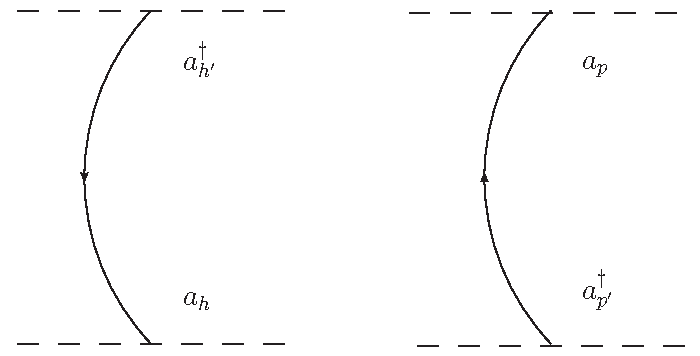
\includegraphics[scale=0.5]{hullpartlinje}
\caption{Diagrammatic representation of the contractions in Eqs. 
\eqref{kontrakt1} and \eqref{kontrakt2} The time is going upward.}
\label{hullpartlinje}
\end{figure}\\
\\
In Fig (\ref{hullpartlinje}) the two contractions in Eqs \eqref{kontrakt1} 
and \eqref{kontrakt2} are represented diagrammatically, the annihilation 
operator $a_\alpha$ destroys the particle line $a^\dagger_\beta$ creates. The
time is upward.\\
\\
With the above definitions of time ordering and contractions we are ready to go back to the time evolution operator, which is already in a time ordered 
form
\be
U(t,t')=\sum_{n=0}^\infty\left(-i\right)^n\int_{t'}^tdt_1
\int_{t'}^{t_1}dt_2\cdots \int_{t'}^{t_{n-1}}dt_nT\left[V(t_1)V(t_2)\cdots V(t_n)\right].
\label{tidevolusjon1}
\ee
From  Eq. \eqref{tidevolusjon1} we see that there are $n!$ ways to order the multidimensional
integral with respect to the times $t_1,t_2 \cdots t_n$, it is again possible to
rewrite the time evolution operator to the form
\be
U(t,t')=\sum_{n=0}^\infty\frac{1}{n!}\left(-i\right)^n\int_{t'}^tdt_1
\int_{t'}^{t}dt_2\cdots \int_{t'}^{t}dt_nT\left[V(t_1)V(t_2)\cdots V(t_n)\right]
\label{tidevolusjon2}
\ee\\
If we recall that it is the energy shift we want to calculate, we can use the 
above equation to write the numerator and the denominator in Eq. 
\eqref{energyshift1} as
\be
%\begin{split}
%&\Delta E_0=\substack{lim\\ \epsilon \rightarrow 0^+}\substack{lim \\t'\rightarrow \\
% -\infty(1-i\epsilon)}\frac{\bra{\phi}VU(0,t')\ket{\phi}}{\bra{\phi}U(0,t')\ket{\phi}}\\
\sum_{n=0}^\infty\frac{1}{n!}\left(-i\right)^n\int_{t'}^tdt_1
\int_{t'}^{t}dt_2\cdots \int_{t'}^{t}dt_n\bra{\phi}T\left[V(t)V(t_1)V(t_2)\cdots V(t_n)\right]\ket{\phi}
\ee
and
\be
 \sum_{n=0}^\infty\frac{1}{n!}\left(-i\right)^n\int_{t'}^tdt_1
\int_{t'}^{t}dt_2\cdots \int_{t'}^{t}dt_n\bra{\phi}T\left[V(t_1)V(t_2)\cdots V(t_n)\right]\ket{\phi}
%\end{split}
%\label{energyshift2}
\ee
respectively.
%Where $V(t)$ in the numerator in  Eq. \eqref{energyshift2} is put into to 
%the time ordering operator. 
To evaluate the integrals in the numerator and the
denominator we have to use Wick's theorem, Wick's theorem with time ordering
will be slightly modified from the first version in section \ref{wicksteorem}. Wicks theorem states now that\\ 
\be
\begin{split}
&T\left[A(t_1)B(t_2)C(t_3) \cdots Z(t_n)\right]=N\left[A(t_1)B(t_2)C(T_3) \cdots Z(t_n)\right]\\
&+ \sum_{1\, contraction}N\left[A(t_1)B(t_2)C(T_3) \cdots Z(t_n)\right]+\sum_{2\, contractions}N\left[A(t_1)B(t_2)C(T_3) \cdots Z(t_n)\right]\\
&+ \cdots + \sum_{\substack{contractions\, with\\ all \, operators}}N\left[A(t_1)B(t_2)C(T_3) \cdots Z(t_n)\right].\\
\end{split}
\label{wicktheofortime}
\ee
Since our unperturbed state is the groundstate, our reference vacuum state, only the last term in Eq. \eqref{wicktheofortime} survives. % We are 
%left with the term where all operators are participating in the contractions. 
Further all unlinked diagrams in the numerator, ie.~all contractions which 
does not include the interaction $V(t)$ are canceled by the diagrams
in the denominator.\\
\\
Let us now evaluate the first-order contribution to the energy shift in Eq. \eqref{energyshift1}. The only contributing term is $V(t)$ which on 
a second quantized form is written as\\ $v_{\alpha\beta\gamma\delta}a^\dagger_\alpha(t) a^\dagger_\beta(t) a_\delta(t) a_\gamma(t).$
From Wick's theorem we will then have two terms contributing to the energy 
shift.
\be
\begin{split}
\wick{21}{<*a^\dagger_\alpha(t) <2a^\dagger_\beta(t) >2 a_\delta(t) >*a_\gamma(t)} +
\wick{21}{<*a^\dagger_\alpha(t) <2a^\dagger_\beta(t) >* a_\delta(t) >2a_\gamma(t)} 
\end{split}
\label{forsteordenbidrag}
\ee
The terms in Eq. \eqref{forsteordenbidrag} can be depicted diagrammatically 
as seen in Fig~\ref{forsteordendiagram}.
\begin{figure}[htp]
\centering
%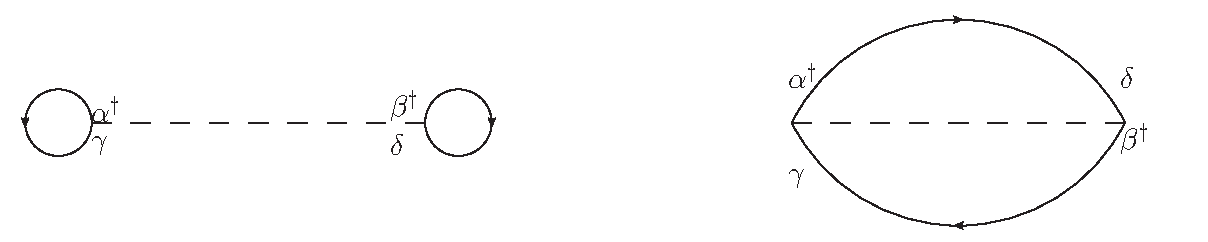
\includegraphics[height=0.8\textheighti]{forsteordendiagram}
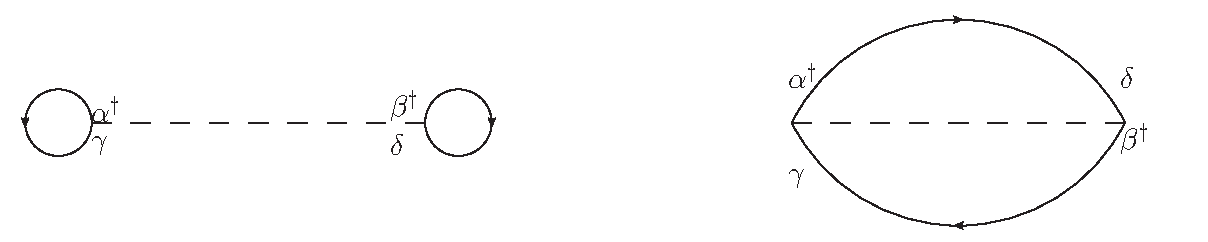
\includegraphics[scale=0.5]{forsteordendiagram}  %[width=1.0\textwidth]{forsteordendiagram}
\caption{Diagrammatic representation of the first order diagram, the diagram to the left depicts the first term in Eq. \eqref{forsteordenbidrag}, the 
diagram to the right depicts the second term in Eq. \eqref{forsteordenbidrag}.}
\label{forsteordendiagram}
\end{figure}
The single particle states $\alpha, \, \beta, \, \gamma$ and $\delta$ must all be holes, since they are all equal time operators.
The energy shift can now be written as 
\be
\Delta E_0=	 \frac{1}{2}\sum_{\alpha\beta < k_f} \frac{1}{2}(v_{\alpha\beta\alpha\beta}-v_{\alpha\beta\beta\alpha}),
\ee
the minus sign comes in, by the "rule" that for every contraction that crosses
another one, contributes with a factor $(-1).$
\begin{figure}[htp]
\centering
%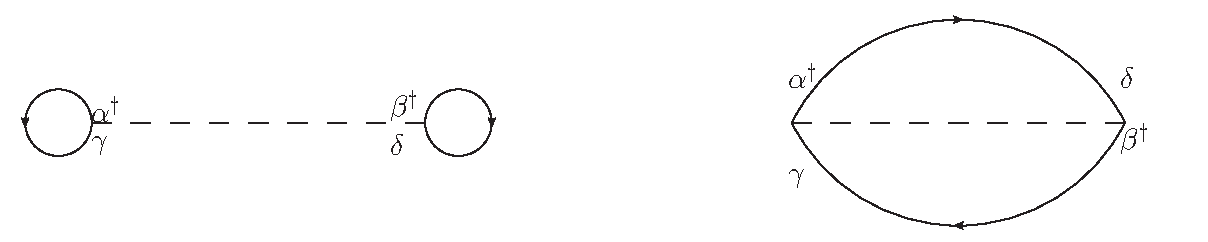
\includegraphics[height=0.8\textheighti]{forsteordendiagram}
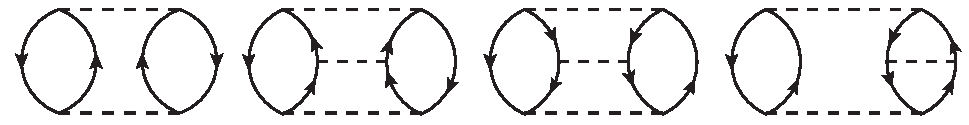
\includegraphics[scale=0.5]{perturbdiag}  %[width=1.0\textwidth]{forsteordendiagram}
\caption{Diagrammatic representation of second to third order contribution to the energy.}
\label{perturbdiagdiagram}
\end{figure}\\
\\
Fig~\ref{perturbdiagdiagram} depicts second- and third-order contributions to
the energy, with the rules for computing the diagrams 
the second order contribution is
\be
\Delta E^{(2)}= \frac{\bra{ij}V\ket{ab}\bra{ab}V\ket{ij}}{\epsilon_{ij}-\epsilon_{ab}},
\ee
where $\epsilon_{pq}=\epsilon_p + \epsilon_q$, denotes the single particle 
energies and the indexes $i$ and $j$ runs over states occupied in the reference vacuum and $a$ and $b$ runs over single-particle states not occupied in the reference vacuum.\\
\\
With the clever invention of diagrams that depict the contractions, we are
able to describe every term in the expansion of the time evolution operator as
diagrams. These diagrams are usually called Feynman diagrams or
Feynman-Goldstone diagrams, to honor the inventors.  When presenting all the
terms as diagrams we need some rules to keep track of them. The idea is that we
find a term in the expansion by studying the corresponding diagram. A nice derivation of the diagram
rules can be found in Ref. \cite{kuo1981}.  The rules are summarized in appendix
\ref{diagramregler}. 




